\chapter{Task-oriented dialog systems}


\section{Human dialogs}

\begin{description}
    \item[Natural language dialog] \marginnote{Natural language dialog}
        Sequence of utterances (i.e., sentences) between two or more participants where each takes a turn.

    \item[Turn-taking problem] \marginnote{Turn-taking problem}
        Determine when the turn of another participant ended.

    \item[Speech/dialog act] \marginnote{Speech/dialog act}
        Indicates the type of utterance.

        \begin{example}
            Yes-no question, declarative question, statement, appreciation, yes answer, \dots
        \end{example}

        \begin{description}
            \item[Adjacency pairs]
                Speech acts that commonly appear together.

                \begin{example}
                    Question $\rightarrow$ answer.
                \end{example}

            \item[Subdialog]
                Dialogs opened and closed within a dialog.

                \begin{example}
                    Correction subdialog, clarification subdialog, \dots
                \end{example}
        \end{description}

    \item[Dialog slot] \marginnote{Dialog slot}
        Relevant entities and properties of an utterance.

        \begin{description}
            \item[Filler] Values assigned to a slot. 
        \end{description}

    \item[Conversation initiative] \marginnote{Conversation initiative}
        Who initiates the dialog.

        \begin{description}
            \item[User initiative]
                The user asks questions and the system responds (e.g., FAQ).

            \item[System initiative]
                The system asks questions to the user (e.g., form completion).

            \item[Mixed initiative]
                Both the user and the system can ask questions.
        \end{description}

    \item[Types of dialog] \marginnote{Types of dialog}
        \phantom{}
        \begin{description}
            \item[Information seeking] To retrieve information.
            \item[Task-oriented] Dialog to achieve a goal.
            \item[Argumentative] Argument in support or against an opinion.
            \item[Explanatory] Teacher-student type of dialog. 
            \item[Recommendation] Persuasion dialog.
            \item[Chit-chat] Free conversation. 
        \end{description}
\end{description}



\section{Task-oriented dialogs}


\subsection{Architectures}

\begin{description}
    \item[Traditional dialog system] \marginnote{Traditional dialog system}
        The main components of an artificial dialog system are:
        \begin{description}
            \item[Natural language understanding (NLU)] \marginnote{Natural language understanding (NLU)}
                Extract the relevant information such as dialog acts and slot-fillers from the utterance.

                \begin{remark}
                    This task can be seen as a named entity recognition problem.
                \end{remark}

                \begin{figure}[H]
                    \centering
                    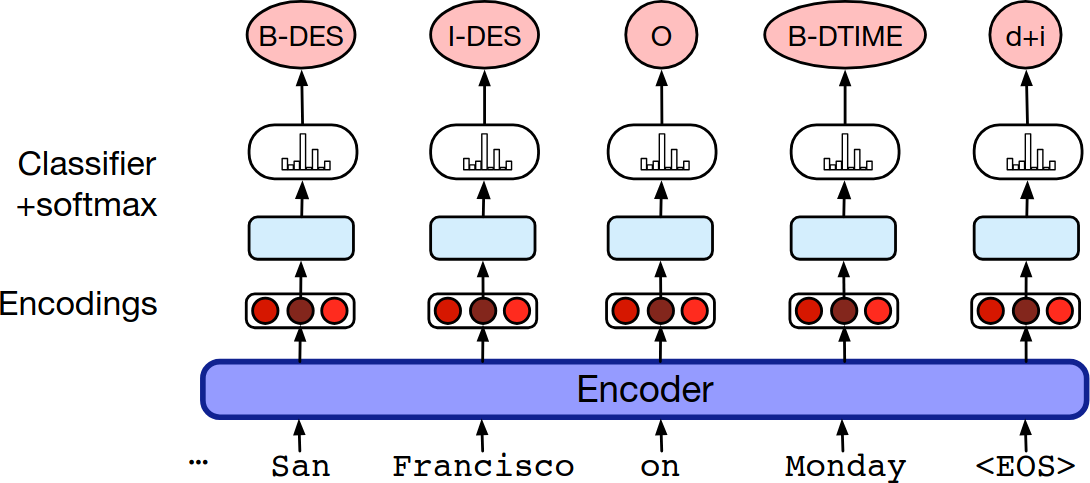
\includegraphics[width=0.45\linewidth]{./img/nlu_arch.png}
                    \caption{Example of neural architecture for slot filling}
                \end{figure}

            \item[Dialog state tracker (DST)] \marginnote{Dialog state tracker (DST)}
                Maintains the history of the dialog. This component should also have access to a knowledge-base.

            \item[Dialog policy manager] \marginnote{Dialog policy manager}
                Produces the dialog acts that composes the response from the output of the DST.

            \item[Natural language generation (NLG)] \marginnote{Natural language generation (NLG)}
                Produces a natural language utterance from the dialog acts produced by the dialog manager.
        \end{description}

        \begin{figure}[H]
            \centering
            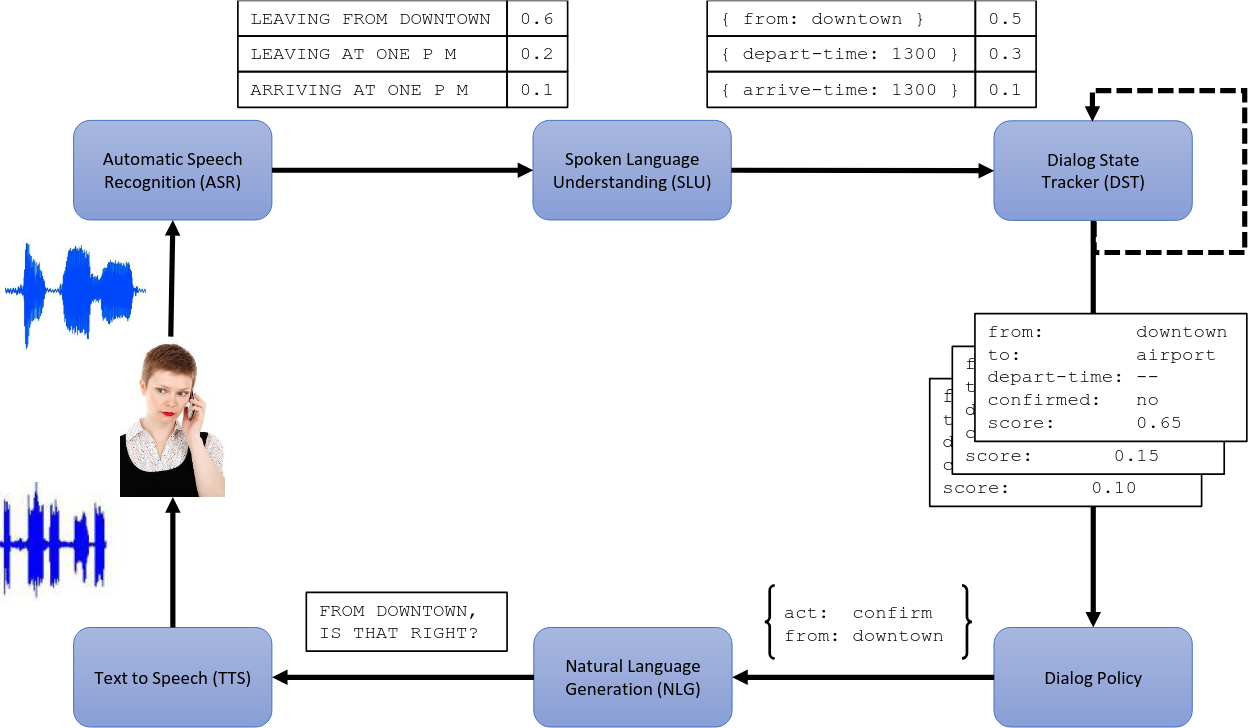
\includegraphics[width=0.85\linewidth]{./img/spoken_dialog_system.png}
            \caption{Example of components for a spoken dialog system}
        \end{figure}


    \item[LLM for dialog system] \marginnote{LLM for dialog system}
        Use a language model that takes as input the utterance and directly produces a response.
\end{description}


\subsection{Dataset}

\begin{description}
    \item[MultiWOZ] \marginnote{MultiWOZ}
        Collection of human-human conversations over multiple domains and topics annotated with dialog states (i.e., turns), slots, and acts.

        The dataset also defines an ontology for slots and a knowledge-base.

        \begin{remark}
            Human annotations are determined by agreement between multiple annotators.
        \end{remark}

        \begin{remark}
            The type of dialogs in the dataset sensibly affects the resulting dialog system.

            \indenttbox
            \begin{example}
                Wizard of Oz collection is a part of MultiWOZ that consists of question-answer dialogs between a user and a wizard. Dialogs produced based on these might result too artificial.
            \end{example}
        \end{remark}
\end{description}



\section{Research topics}


\subsection{LLM domain portability}

\begin{description}
    \item[Domain portability] \marginnote{Domain portability}
        Adapt a model to a new domain (i.e., knowledge-base).

        Possible approaches are:
        \begin{descriptionlist}
            \item[Fine-tuning] 
                Fine-tune the LLM with the new knowledge-base.

                \begin{remark}
                    This approach is susceptible to the catastrophic forgetting problem.
                \end{remark}

            \item[Prompting] 
                Embed the new knowledge-base into the prompt of the LLM.

                \begin{remark}
                    This approach risks hallucinations and is constrained to the limits of the context length and computational inefficiency.
                \end{remark}

            \item[Functional calling] 
                Let the LLM query the knowledge-base when needed.

                \begin{remark}
                    This approach requires more complex prompts and not all LLMs support it.
                \end{remark}
            \end{descriptionlist}

        \begin{remark}
            Experimental results show that functional calling works better than embedding the KB in the prompt. It is also more effective when the KB becomes bigger.
        \end{remark}
\end{description}


\subsection{LLM pragmatics}

\begin{description}
    \item[Pragmatics] \marginnote{Pragmatics}
        Ability to adapt a conversation based on the context.

    \item[Proactivity] \marginnote{Proactivity}
        Ability of providing useful but not explicitly requested information.

        \begin{remark}
            An LLM can be made more proactive by prompting or fine-tuning.
        \end{remark}
\end{description}


\subsection{LLM for dialog generation}

\begin{description}
    \item[Automatic dialog generation] \marginnote{Automatic dialog generation}
        Use an LLM to generate and annotate dialogs to create a synthetic dataset. A possible approach is based on the following steps:
        \begin{descriptionlist}
            \item[Generation] 
                Use the LLM to generate a dialog. Possible approaches are:
                \begin{descriptionlist}
                    \item[One-pass] Prompt the LLM to generate a dialog based on a few references.
                    \item[Interactive] Produce a dialog by conversing with the model.
                    \item[Teacher-student] Let two LLMs converse.
                \end{descriptionlist}

            \item[Annotation] 
                Prompt the LLM to annotate the generated dialog based on some schema.

            \item[Evaluation] 
                Evaluate based on human opinion.
        \end{descriptionlist}
\end{description}